% \documentclass{article}
% \usepackage{beamerarticle}
\documentclass{beamer}
% Beamer theme settings
\usetheme{Madrid}
\usecolortheme{default}
\usepackage{amsmath}

\usepackage{tikz}
\usetikzlibrary{intersections}

% Define commands for vectors
\newcommand{\va}{\mathbf{a}}
\newcommand{\vb}{\mathbf{b}}
\newcommand{\vc}{\mathbf{c}}
\newcommand{\vd}{\mathbf{d}}
\newcommand{\ve}{\mathbf{e}}
\newcommand{\vv}{\mathbf{v}}
\newcommand{\vu}{\mathbf{u}}
\newcommand{\vw}{\mathbf{w}}
\newcommand{\vx}{\mathbf{x}}
\newcommand{\vy}{\mathbf{y}}
\newcommand{\vz}{\mathbf{z}}
\newcommand{\N}{\mathbb{N}}
\newcommand{\Z}{\mathbb{Z}}
\newcommand{\R}{\mathbb{R}}
\newcommand{\Q}{\mathbb{Q}}



% Title page

\title[Lecture 1]{Vectors}
\author[Aprikyan, Tarkhanyan]{Hayk Aprikyan, Hayk Tarkhanyan}
\institute[ACA]{Armenian Code Academy}
\date{March 18, 2025}

\begin{document}

\begin{frame}
  \titlepage
\end{frame}

\begin{frame}
\begin{itemize}
    % \item Schedule:
    % \begin{itemize}
    %     \item Monday: 20:00--22:00
    %     \item Thursday: 20:00--22:00
    %     \item Saturday: 12:00--14:00
    % \end{itemize}
    % \medskip
    \item Communication:
    \begin{itemize}
        \item For questions, memes, announcements, homeworks: Slack
        \item For lecture slides and books: Google Drive, GitHub
    \end{itemize}
    \medskip
    
    \item Main books (in English):

    \begin{itemize}
        \item Deisenroth, "Mathematics for Machine Learning"
        \item Poole, "Linear Algebra: A Modern Introduction"
        \item Strang, "Introduction to Linear Algebra"
        \item Mikaelian, "Linear Algebra: Theorems and Algorithms"
        \item Grimmett, Welsh, "Probability: An Introduction"
        \item Stewart, "Calculus"
\end{itemize}
    \item Supplementary books (in Armenian):
    
\begin{itemize}
        \item Ohanyan, "Probability Theory", Lectures
        \item Gevorgyan, Sahakyan, "Algebra and Elements of Mathematical Analysis 11, 12" 
        \item Musoyan, "Mathematical Analysis", parts 1-2 
        \item Movsisyan, "Higher Algebra and Number Theory" 
    \end{itemize}

    
\end{itemize}

\end{frame}

% Slide 1: coins
\begin{frame}{Vectors}
  \begin{itemize}
    \item<1-> Suppose one has 2 x 10 dram, 1 x 20 dram, 2 x 50 dram, and 1 x 200 dram coins in his pocket.
    \item<2-> How can we denote that?
    \item<3-> Using a table: \begin{table}[h]
      % \centering
      \raggedright
      \begin{tabular}{|c|c|}
        \hline
        \textbf{Coins} & \textbf{Quantity} \\
        \hline
        10 & 2\\
        \hline
        20 & 1\\
        \hline
        50 & 2 \\
        \hline
        100 & 0 \\
        \hline
        200 & 1 \\
        \hline
      \end{tabular}
      \label{tab:coins}
    \end{table}
    \item<4-> Or by taking the two columns of the table: $\begin{bmatrix}
10 \\ 20 \\ 50 \\ 100 \\ 200
\end{bmatrix}$, $\begin{bmatrix}
2 \\1 \\2 \\0 \\1 \\
\end{bmatrix}$
  \end{itemize}
\end{frame}

% Slide 2: Definition
\begin{frame}{Vectors}
  \begin{block}{Definition}
  An ordered set of \( n \) real numbers is called a \textbf{vector} (or \textbf{column vector}) in \( \mathbb{R}^n \):
  
  \[
  \mathbf{v} = \begin{bmatrix} v_1 \\ v_2 \\ \vdots \\ v_n \end{bmatrix}
  \]

  where \( v_1, v_2, \ldots, v_n \) are the \textbf{components} of the vector.

  A vector written horizontally is called a \textbf{row vector}:
  \[\mathbf{v} = \begin{bmatrix} v_1 & v_2 & \ldots & v_n \end{bmatrix}\]
\end{block}

We will denote $\mathbf{v} \in \mathbb{R}^n$ to indicate that $v$ is a vector in \( \mathbb{R}^n \).

\pause Vectors in $\mathbb{R}^1$ \pause are real numbers: $[v]\in\mathbb{R}$.
  \end{frame}

% Slide 3: Examples
\begin{frame}{Examples of Vectors in \( \mathbb{R}^n \)}
  \begin{align*}
    \mathbf{v}_1 &= \begin{bmatrix} 2 \\ -1 \\ 0 \end{bmatrix} \quad \text{(3-dimensional column vector)} \\
    \mathbf{v}_2 &= \begin{bmatrix} 1 \\ 1 \\ 1 \\ 1 \end{bmatrix} \quad \text{(4-dimensional column vector)} \\
    \mathbf{v}_3 &= \begin{bmatrix} -3 \\ 2 \end{bmatrix} \quad \text{(2-dimensional column vector)} \\
    \mathbf{v}_4 &= \begin{bmatrix} 0 \\ 0 \\ 0 \end{bmatrix} \quad \text{(Zero vector in 3-dimensional space)} \\
    \mathbf{v}_5 &= \begin{bmatrix} 1 & -1 & 2 \end{bmatrix} \quad \text{(3-dimensional row vector)}
  \end{align*}
\end{frame}


% Slide 4: Addition
\begin{frame}{Addition of vectors}
Let's denote $\mathbf{a} = \begin{bmatrix}
10 \\ 20 \\ 50 \\ 100 \\ 200
\end{bmatrix}$, $\mathbf{b} = \begin{bmatrix}
2 \\1 \\2 \\0 \\1 \\
\end{bmatrix}.$ \pause $\mathbf{a},\mathbf{b} \in \mathbb{R}^5$.
\pause What if someone gave us $3 \times 100$ drams and $1 \times 200$ drams?
\pause Denote $\mathbf{c} = \begin{bmatrix}
0 \\ 0 \\ 0 \\ 3 \\ 1
\end{bmatrix}$.\\
\pause We would have the following coins:
\[
\mathbf{b} + \mathbf{c} = \begin{bmatrix}
2 \\1 \\2 \\0 \\1 \\
\end{bmatrix} + \begin{bmatrix}
0 \\ 0 \\ 0 \\ 3 \\ 1
\end{bmatrix} = \begin{bmatrix}
2+0 \\ 1+0 \\ 2+0 \\ 0+3 \\ 1+1
\end{bmatrix} = \begin{bmatrix}
2 \\ 1 \\ 2 \\ 3 \\ 2
\end{bmatrix}
\]
\end{frame}


% Slide 5: Addition
\begin{frame}{Addition of vectors}
  \begin{block}{Definition}
  To add two vectors \( \mathbf{v} = \begin{bmatrix} v_1 \\ v_2 \\ \vdots \\ v_n \end{bmatrix} \) and \( \mathbf{u} = \begin{bmatrix} u_1 \\ u_2 \\ \vdots \\ u_n \end{bmatrix} \) in \( \mathbb{R}^n \), add their corresponding components:
  \begin{align*}
    \mathbf{v} + \mathbf{u} &= \begin{bmatrix} v_1 + u_1 \\ v_2 + u_2 \\ \vdots \\ v_n + u_n \end{bmatrix}
  \end{align*}
\end{block}

\pause Note that we can only add two vectors if they are of the same length!

\end{frame}


% Slide 6: Multiplication by scalar
\begin{frame}{Multiplication of vector by scalar}
What if the money in our pockets doubled? 
\pause We would have:
$$2 \cdot \mathbf{b} = 2\cdot \begin{bmatrix}
2 \\1 \\2 \\0 \\1 \\
\end{bmatrix} = \begin{bmatrix}
4 \\2 \\4 \\0 \\2 \\
\end{bmatrix} $$
from each coin.

\end{frame}


% Slide 7: Def
\begin{frame}{Multiplication of vector by scalar}

  \begin{block}{Definition}
    To multiply a vector \( \mathbf{v} = \begin{bmatrix} v_1 \\ v_2 \\ \vdots \\ v_n \end{bmatrix} \) by a scalar \( c \) in \( \mathbb{R}^n \), multiply each component of the vector by the scalar:

  \begin{align*}
    c \cdot \mathbf{v} &= \begin{bmatrix} c \cdot v_1 \\ c \cdot v_2 \\ \vdots \\ c \cdot v_n \end{bmatrix}
  \end{align*}
\end{block}
\end{frame}

% Slide 8: Properties of Vectors
\begin{frame}{Properties of Vectors}
  \begin{block}{Associativity and Commutativity of Vector Addition}
    For any vectors \( \mathbf{u} \) and \( \mathbf{v} \) in \( \mathbb{R}^n \), the vector addition is commutative and associative:
    $$    \mathbf{u} + \mathbf{v} = \mathbf{v} + \mathbf{u}$$
    $$    (\mathbf{u} + \mathbf{v}) + \mathbf{w} = \mathbf{u} + (\mathbf{v} + \mathbf{w})$$
  \end{block}

\pause  \begin{block}{Associativity and Commutativity of Scalar Multiplication}
    For any scalar \( c \) and vectors \( \mathbf{v} \) and \( \mathbf{u} \) in \( \mathbb{R}^n \), scalar multiplication is associative and commutative:
$$    c \cdot (\mathbf{v} + \mathbf{u}) = c \cdot \mathbf{v} + c \cdot \mathbf{u}$$
$$    (c \cdot d) \cdot \mathbf{v} = c \cdot (d \cdot \mathbf{v})$$
  \end{block}
\end{frame}

% Slide 9: -
\begin{frame}{Vector Subtraction}
What if we take a bus and spend 2 x 50 drams?
\pause  \begin{block}{Definition}
    For a vector \( \mathbf{v} = \begin{bmatrix} v_1 \\ v_2 \\ \vdots \\ v_n \end{bmatrix} \) in \( \mathbb{R}^n \), the \textbf{negative} of \( \mathbf{v} \), denoted as \( -\mathbf{v} \), is obtained by negating each component:

    \[
    -\mathbf{v} = \begin{bmatrix} -v_1 \\ -v_2 \\ \vdots \\ -v_n \end{bmatrix}
    \]
  \end{block}
\end{frame}

% Slide 9.5: -
\begin{frame}{Vector Subtraction}


  \begin{block}{Vector Subtraction}
    The subtraction of vectors \( \mathbf{u}  \) and \( \mathbf{v} \) in \( \mathbb{R}^n \) is defined as the sum of \( \mathbf{u} \) and the negative of \( \mathbf{v} \):

    \[
    \mathbf{u} - \mathbf{v} = \mathbf{u} + (-\mathbf{v}) = \begin{bmatrix} u_1 - v_1 \\ u_2 - v_2 \\ \vdots \\ u_n - v_n \end{bmatrix}
    \]
  \end{block}

  \pause\begin{exampleblock}{Example}
    \[
    \begin{bmatrix} 2 \\ -1 \\ 3 \end{bmatrix} - \begin{bmatrix} 1 \\ 4 \\ 0 \end{bmatrix} = \begin{bmatrix} 2 - 1 \\ -1 - 4 \\ 3 - 0 \end{bmatrix} = \begin{bmatrix} 1 \\ -5 \\ 3 \end{bmatrix}
    \]
  \end{exampleblock}
\end{frame}

% Slide 10: T
\begin{frame}{Vector Transposition}
  \begin{block}{Definition}
    For a column vector \( \mathbf{v} = \begin{bmatrix} v_1 \\ v_2 \\ \vdots \\ v_n \end{bmatrix} \) in \( \mathbb{R}^n \), the \textbf{transpose}, denoted as \( \mathbf{v}^T \), is a row vector:
    
    \[
    \mathbf{v}^T = \begin{bmatrix} v_1 & v_2 & \cdots & v_n \end{bmatrix}
    \]
    
    \pause For a row vector \( \mathbf{u} = \begin{bmatrix} u_1 & u_2 & \cdots & u_n \end{bmatrix} \) in \( \mathbb{R}^n \), the \textbf{transpose}, denoted as \( \mathbf{u}^T \), is a column vector:
    
    \[
    \mathbf{u}^T = \begin{bmatrix} u_1 \\ u_2 \\ \vdots \\ u_n \end{bmatrix}
    \]
  \end{block}

\end{frame}


% Slide 11: T properties
\begin{frame}{Vector Transposition}
  Examples:
    \[
    \begin{bmatrix} 2 \\ -1 \\ 3 \end{bmatrix}^T = \begin{bmatrix} 2 & -1 & 3 \end{bmatrix}
    \]
    
   \pause \[
    \begin{bmatrix} 1 & 0 & -2 \end{bmatrix}^T =\pause \begin{bmatrix} 1 \\ 0 \\ -2 \end{bmatrix}
    \]
  
  \pause\begin{block}{Transpose Properties}
    \begin{itemize}
      \item For any vector \( \mathbf{v} \) in \( \mathbb{R}^n \), \( (\mathbf{v}^T)^T = \mathbf{v} \)
      \item For any scalar \( c \), \( (c \cdot \mathbf{v})^T = c \cdot \mathbf{v}^T \)
    \end{itemize}
  \end{block}

\end{frame}


% Slide 13: Dot prod
\begin{frame}{Dot Product of Vectors}
In our example we had $\mathbf{b} = \begin{bmatrix}
2 \\1 \\2 \\0 \\1 \\
\end{bmatrix}$ coins of  $\mathbf{a} = \begin{bmatrix}
10 \\ 20 \\ 50 \\ 100 \\ 200
\end{bmatrix}$ nominations (values) respectively.

\pause How much money do we have in total?

\pause   \begin{block}{Definition}
    The \textbf{dot product} of two vectors \( \mathbf{u} = \begin{bmatrix} u_1 \\ u_2 \\ \vdots \\ u_n \end{bmatrix} \) and \( \mathbf{v} = \begin{bmatrix} v_1 \\ v_2 \\ \vdots \\ v_n \end{bmatrix} \) in \( \mathbb{R}^n \) is:

    \[
    \mathbf{u} \cdot \mathbf{v} = u_1 \cdot v_1 + u_2 \cdot v_2 + \cdots + u_n \cdot v_n
    \]
  \end{block}

\end{frame}

% Slide 14: Dot prod examples
\begin{frame}{Dot Product of Vectors}
  \begin{exampleblock}{Example}
    If \( \mathbf{u} = \begin{bmatrix} 2 \\ -1 \\ 3 \end{bmatrix} \) and \( \mathbf{v} = \begin{bmatrix} 1 \\ 4 \\ 0 \end{bmatrix} \), then:

    \[
    \mathbf{u} \cdot \mathbf{v} = (2 \cdot 1) + (-1 \cdot 4) + (3 \cdot 0) = 2 - 4 + 0 = -2
    \]
  \end{exampleblock}
\pause Going back to our example, we can calculate our money with the dot product of $\mathbf{a}$ and $ \mathbf{b}$:
$$\mathbf{a} \cdot \mathbf{b}= \begin{bmatrix}
2 \\1 \\2 \\0 \\1 \\
\end{bmatrix}\cdot \begin{bmatrix}
10 \\ 20 \\ 50 \\ 100 \\ 200
\end{bmatrix} = 2 \cdot 10 + 1 \cdot 20 + 2 \cdot 50 + 0 \cdot 100 + 1\cdot 200 = 340$$

\end{frame}


% Slide 15: Dot prod
\begin{frame}{Dot Product of Vectors}
  \begin{block}{Remark 1}
    The dot product of two vectors is defined if and only if the vectors have the same number of components (i.e. are of the same length).
  \end{block}

  \begin{block}{Remark 2}
    The dot product of two vectors is a \textit{number} (scalar), not a vector.
  \end{block}

  \pause This is why the dot product is often called \textbf{scalar product}.

\end{frame}


% Slide 16: Properties of Dot prod 
\begin{frame}{Properties of Dot Product}
  \begin{block}{Properties}
    Let \( \mathbf{u} \), \( \mathbf{v} \), and \( \mathbf{w} \) be vectors in \( \mathbb{R}^n \), and let \( c \) be a scalar. The dot product has the following properties:

    \begin{enumerate}
      \item {Commutativity:} $$ \mathbf{u} \cdot \mathbf{v} = \mathbf{v} \cdot \mathbf{u}$$
      \item {Distributivity over Vector Addition:} $$ (\mathbf{u} + \mathbf{v}) \cdot \mathbf{w} = \mathbf{u} \cdot \mathbf{w} + \mathbf{v} \cdot \mathbf{w} $$
      \item {Scalar Multiplication:} $$(c \cdot \mathbf{u}) \cdot \mathbf{v} = c \cdot (\mathbf{u} \cdot \mathbf{v}) = \mathbf{u} \cdot (c \cdot \mathbf{v})$$
      \item {Non-negativity:} 
      
      \centerline{$\mathbf{u} \cdot \mathbf{u} \geq 0 $ and \( \mathbf{u} \cdot \mathbf{u} = 0 \) if and only if \( \mathbf{u} = \mathbf{0} \)}
    \end{enumerate}
  \end{block}
\end{frame}

% Slide 17: More examples
\begin{frame}{Examples}
  Consider vectors \( \mathbf{u} = \begin{bmatrix} 1 \\ -2 \\ 3 \end{bmatrix} \), \( \mathbf{v} = \begin{bmatrix} 0 \\ 4 \\ -1 \end{bmatrix} \), and \( \mathbf{w} = \begin{bmatrix} -2 \\ 1 \\ 2 \end{bmatrix} \).

  Let's calculate \( (5\mathbf{u} - \mathbf{v}) \cdot \mathbf{w} \):

  \pause  
  \begin{align*}
      (5\mathbf{u} - \mathbf{v}) \cdot \mathbf{w} &= \left(5\cdot\begin{bmatrix} 1 \\ -2 \\ 3 \end{bmatrix} - \begin{bmatrix} 0 \\ 4 \\ -1 \end{bmatrix}\right) \cdot \begin{bmatrix} -2 \\ 1 \\ 2 \end{bmatrix} \\&= \left(\begin{bmatrix} 5 \\ -10 \\ 15 \end{bmatrix} - \begin{bmatrix} 0 \\ 4 \\ -1 \end{bmatrix}\right) \cdot \begin{bmatrix} -2 \\ 1 \\ 2 \end{bmatrix} 
      \\&= \begin{bmatrix} 5 \\ -14 \\ 16 \end{bmatrix} \cdot \begin{bmatrix} -2 \\ 1 \\ 2 \end{bmatrix} = 5 \cdot (-2) + (-14) \cdot 1 + 16 \cdot 2 = 8  \end{align*}
    
\end{frame}



% Slide 4: geometric interpretation
\begin{frame}{Geometric interpretation of vectors}

  \begin{itemize}[<+->]
    \item So far, we were treating vectors in $\mathbb{R}^n$ as lists of numbers only.
    \item For example: $\vv=\begin{bmatrix}2\\3    \end{bmatrix}$, a 2-dimensional column vector.
  \end{itemize}

  \pause

  \begin{block}{Geometric Interpretation}
    \begin{itemize}
      \item In addition to their algebraic representation, vectors have a geometric interpretation.
      \item We can think of a vector $\mathbf{v}$ as a point in the 2d space,
      
      \item Or we can imagine it as an arrow in space, starting from the origin ($O(0,0)$) and pointing to the mentioned point.
      \item The components of $\vv$ are the \textbf{coordinates} of the point in the plane.
    \end{itemize}
  \end{block}
\end{frame}





% Slide 5: geometric interpretation
\begin{frame}{Geometric interpretation of vectors}
  \begin{example}
    \begin{columns}
      \begin{column}{0.5\textwidth}
        \begin{itemize}
          \item Consider the vector $\mathbf{v} = \begin{bmatrix} 2 \\ 3 \end{bmatrix}$.
          \item This vector points to the point (2, 3) in the plane.
        \end{itemize}
      \end{column}
      \begin{column}{0.5\textwidth}
        \begin{center}
          \begin{tikzpicture}[scale=0.8]
            \draw[->] (0,0) -- (2,3) node[midway, above left] {$\mathbf{v}$};
            \draw[dashed] (0,0) -- (2,0) node[midway, below] {$2$};
            \draw[dashed] (2,0) -- (2,3) node[midway, right] {$3$};
          \end{tikzpicture}
        \end{center}
      \end{column}
    \end{columns}
  \end{example}

  In general, the vector with coordinates $\begin{bmatrix}
      x\\y
  \end{bmatrix}$ is represented by the point with coordinates $(x,y)$.\\
  \\
  \\
\pause What do you think happens in the 3d space?

  \end{frame}




% Slide 6: Addition
\begin{frame}{Addition of vectors}
Let's interpret some of our vector operations geometrically.

    \begin{itemize}
      \item \textbf{Addition:} To add vectors $\mathbf{u}$ and $\mathbf{v}$, place the tail of $\mathbf{v}$ at the head of $\mathbf{u}$. The sum $\mathbf{u} + \mathbf{v}$ is the vector pointing from the tail of $\mathbf{u}$ to the head of $\mathbf{v}$.
    \end{itemize}

    \begin{center}
      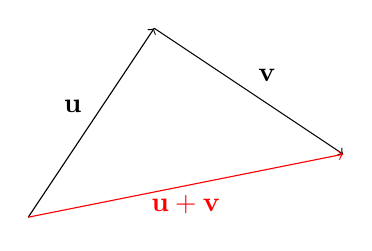
\begin{tikzpicture}[scale=0.8]
        \draw[->] (0,0) -- (2,3) node[midway, above left] {$\mathbf{u}$};
        \draw[->] (2,3) -- (5,1) node[midway, above right] {$\mathbf{v}$};
        \draw[->,red] (0,0) -- (5,1) node[midway, below] {$\mathbf{u} + \mathbf{v}$};
      \end{tikzpicture}
    \end{center}

\end{frame}


% Slide 7: negative
\begin{frame}{Negative of vectors}
    \begin{itemize}
      \item \textbf{Negation:} The negative of a vector $\mathbf{v}$, denoted $-\mathbf{v}$, is a vector with the same magnitude but opposite direction.
    \end{itemize}

    \begin{center}
      \begin{tikzpicture}[scale=0.8]
        \draw[->] (0,0) -- (2,3) node[midway, above left] {$\mathbf{v}$};
        \draw[->,blue] (0,0) -- (-2,-3) node[midway, below] {$-\mathbf{v}$};
      \end{tikzpicture}
    \end{center}

\end{frame}


% Slide 7: -
\begin{frame}{Subtraction of vectors}
    \begin{itemize}
      \item \textbf{Subtraction:} To subtract $\mathbf{v}$ from $\mathbf{u}$, place the tail of $\mathbf{v}$ at the head of $\mathbf{u}$. The result $\mathbf{u} - \mathbf{v}$ is the vector pointing from the head of $\mathbf{v}$ to the head of $\mathbf{u}$.
    \end{itemize}

    \begin{center}
      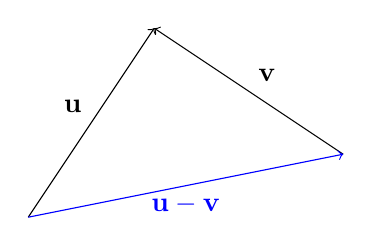
\begin{tikzpicture}[scale=0.8]
        \draw[->] (0,0) -- (2,3) node[midway, above left] {$\mathbf{u}$};
        \draw[->] (5,1) -- (2,3) node[midway, above right] {$\mathbf{v}$};
        \draw[->,blue] (0,0) -- (5,1) node[midway, below] {$\mathbf{u} - \mathbf{v}$};
      \end{tikzpicture}
    \end{center}
\end{frame}


% Slide 9: *
\begin{frame}{Multiplication by scalar}
    \begin{itemize}
      \item \textbf{Scalar Multiplication:} Scaling a vector $\mathbf{v}$ by a scalar $c$ stretches or compresses the vector. The result $c \cdot \mathbf{v}$ has the same direction as $\mathbf{v}$ but a different magnitude.
    \end{itemize}

    \begin{center}
      \begin{tikzpicture}[scale=0.8]
        \draw[->] (0,0) -- (2,3) node[midway, above left] {$\mathbf{v}$};
        \draw[->,red] (0,0) -- (4,6) node[near end, above left] {$2 \cdot \mathbf{v}$};
      \end{tikzpicture}
    \end{center}
\end{frame}

% Slide 10: example
\begin{frame}{Example}

  \begin{example}
    Let \( \mathbf{a} = [3, 2]\) and \( \mathbf{b} = [2, 0] \). We want to find \( 3\mathbf{a} + \mathbf{b} \).
  \end{example}

  \pause

  \begin{block}{Vector Operations}
    \begin{itemize}
      \item \( 3\mathbf{a} + \mathbf{b} = 3 \cdot [3, 2] + [2, 0] \)
      \item \( 3\mathbf{a} + \mathbf{b} = [9,6] + [2, 0] \)
      \item \( 3\mathbf{a} + \mathbf{b} = [11, 6] \)
    \end{itemize}
  \end{block}

  \pause
How can we interpret it geometrically?

\end{frame}


% Slide 10: example
\begin{frame}{Example}
  \begin{center}
    \begin{tikzpicture}[scale=0.8]
      \draw[->,white] (0,0) -- (11,6) node[midway, below] {$3\mathbf{a} + \mathbf{b}$};
      \draw[->] (0,0) -- (3,2) node[midway, above left] {$\mathbf{a}$};
      \draw[->] (0,0) -- (2,0) node[midway, below] {$\mathbf{b}$};
    \end{tikzpicture}
  \end{center}
\end{frame}
\begin{frame}{Example}
  \begin{center}
    \begin{tikzpicture}[scale=0.8]
      \draw[->,white] (0,0) -- (11,6) node[midway, below] {$3\mathbf{a} + \mathbf{b}$};
      \draw[->] (0,0) -- (3,2) node[midway, above left] {$\mathbf{a}$};
      \draw[->] (0,0) -- (2,0) node[midway, below] {$\mathbf{b}$};
      \draw[->] (0,0) -- (9,6) node[midway, right] {$3\mathbf{a}$};
    \end{tikzpicture}
  \end{center}
\end{frame}
\begin{frame}{Example}
  \begin{center}
    \begin{tikzpicture}[scale=0.8]
      \draw[->,white] (0,0) -- (11,6) node[midway, below] {$3\mathbf{a} + \mathbf{b}$};
      \draw[->] (0,0) -- (3,2) node[midway, above left] {$\mathbf{a}$};
      \draw[->] (0,0) -- (2,0) node[midway, below] {$\mathbf{b}$};
      \draw[->] (0,0) -- (9,6) node[midway, right] {$3\mathbf{a}$};
      \draw[->] (9,6) -- (11,6) node[midway, below] {$\mathbf{b}$};
    \end{tikzpicture}
  \end{center}
\end{frame}\begin{frame}{Example}
  \begin{center}
    \begin{tikzpicture}[scale=0.8]
      \draw[->] (0,0) -- (3,2) node[midway, above left] {$\mathbf{a}$};
      \draw[->] (0,0) -- (2,0) node[midway, below] {$\mathbf{b}$};
      \draw[->] (0,0) -- (9,6) node[midway, right] {$3\mathbf{a}\quad \quad $};
      \draw[->] (9,6) -- (11,6) node[midway, below] {$\mathbf{b}$};
      \draw[->,red] (0,0) -- (11,6) node[midway, below] {\;\;\;\;\;\;\;\;$3\mathbf{a} + \mathbf{b}$};
    \end{tikzpicture}
  \end{center}
  
\end{frame}



\end{document}
